\section{Introduction}
Data are susceptible to various forms of corruption such as missing, incorrect, or inconsistent values.
Predictive modeling, such as regression and classification, is an increasingly popular form of analytics \cite{bdas, alexandrov2014stratosphere, crotty2014tupleware, hellerstein2012madlib}.
These models rely on learning relationships between features and labels, and systematic corruption \cite{taylor1982introduction} can affect these relationships.
The high dimensionality of these models can amplify small problems resulting in error-prone predictions even when trained on mostly correct data \cite{xiaofeature}.
Consequently, some form of data cleaning or pre-processing is usually applied before predictive modeling to provide clean training data.

In some cases, it may be obvious that a record is corrupted (e.g., missing values), and without appropriate error-handling any analysis would fail.
However, there are a number of interesting cases where data are subtly corrupted and at first glance may look like consistent database records~\cite{rahm2000data}.
For example, battery-powered sensors can transmit unreliable measurements when battery levels are low \cite{DBLP:conf/pervasive/JefferyAFHW06}. 
Similarly, data entered by humans can be susceptible to a variety of inconsistencies (e.g., typos), and unintentional cognitive biases~\cite{DBLP:conf/recsys/KrishnanPFG14}.
Such errors are particularly problematic since the analysts code may run perfectly, but produces an inaccurate model that mis-predicts some subpopulations of data.
Furthermore, the consequences of an inaccurate model may be only be apparent when the model is deployed and queried in the future. 

Detecting these hidden, yet possibly significant, errors is an inherently iterative process~\cite{dasu2003exploratory} that often requires training the complete model and identifying data that are not predicted well.
Once some dirty data are identified, the analyst must decide how to handle the corruption (e.g., repair or remove). 
The analyst iterates in a time-consuming train, clean, and re-train loop until she is sufficiently confident in the model's accuracy.
As datasets grow and models become more complex, it is impractical to expect analysts to verify every record in a large dataset or enumerate every possible type of error.
Then, the fundemental question is whether it is possible to train an accurate model while only cleaning $k \ll N$ records in a dataset. 
This paper presents a framework called \sys to support this iterative cleaning and training process by providing efficient prioritization of records to check and reliable estimates of the accuracy of intermediate results.

\sys is inspired by the recent success of progressive data cleaning where a user can gradually clean more data until the desired accuracy is reached~\cite{altowim2014progressive, whang2014incremental, papenbrock2015progressive, gruenheid2014incremental, mayfield2010eracer, DBLP:journals/pvldb/YakoutENOI11, yakout2013don}.
Similarly, we explore the problem of progressive cleaning with model training, where as more data are cleaned, the effects of systematic error in a model are gradually reduced.
Designing such a framework is challenging since the straight-forward integration of data cleaning and model training can result in highly inaccurate models.
For example, one could repair the first $k$ dirty records in place, and re-train the user's model after each repair.
While intuitive, we show that mixing dirty and clean training data can lead to misleading results even in simple scenarios (Figure \ref{update-arch1}).
An alternative is to restrict training to just the $k$ clean records (e.g., sampling \cite{wang1999sample}).
While this approach avoids the mixing problem, accurate model training may require a large amount of training data and $k$ examples may not be enough for a viable model.
Furthermore, if the $k$ records are not selected uniformly at random, the trained model might be highly biased.
The errors and inefficiencies introduced by these three problems may dominate any gains from data cleaning, leading to unreliable or misleading conclusions about data or model quality.

\begin{figure}[t]
\centering
 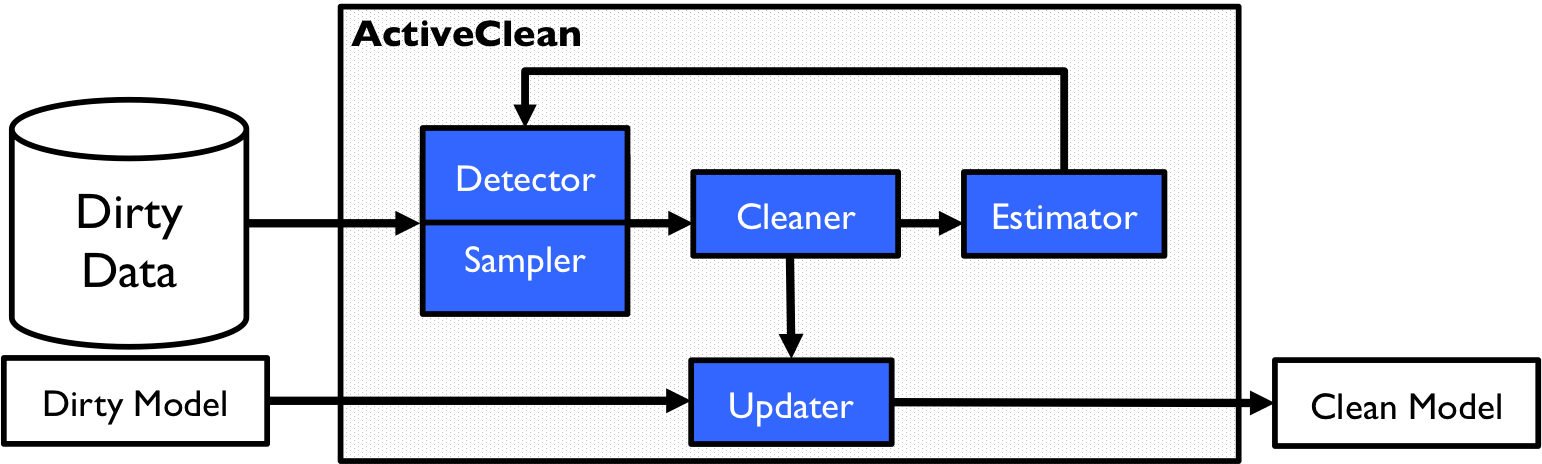
\includegraphics[width=\columnwidth]{figs/arch.png}
 \caption{\sysfull allows users to train predictive models while progressively cleaning data. The framework adaptively selects the best data to clean and can optionally (denoted with dotted lines) integrate with pre-defined detection rules and estimation algorithms for improved conference. \label{sys-arch}}\vspace{-2em}
\end{figure}

Consequently, while there is extensive work on progressive data cleaning before analysis, due to the aforementioned problems, existing tools are not suited for application inside the cleaning and training loop.  
To this end, we designed \sys which trains predictive models with progressive data cleaning and has accuracy guarantees.
We focus on a popular class of models called convex loss models (e.g., includes linear regression and SVMs).
We show that instead of re-training the model, the model can be initialized by training on the dirty data and then iteratively corrected as more data are cleaned.
The iterative corrections, which use gradient descent, provide guarantees that allow analysts to trust early results and make predictions using the model.
Intuitively, this process leverages the convex structure of the model rather than treating it like a black-box, and we can apply convergence arguments from standard convex optimization theory.
We also propose several novel optimizations that leverage information from the model to guide data cleaning towards the records most likely to be dirty and most likely to affect the results.

%High-dimensional predictive models are highly sensitive to dirty data.
%They rely on learning relationships between features and labels, and systematic data corruption \cite{taylor1982introduction} can mask or even introduce spurious new relationships.
%Furthermore, the high dimensionality of these models can amplify small problems \cite{xiaofeature} resulting in error-prone predictions even when trained on mostly clean data.





%When data cleaning is expensive, it is desirable to apply it \textbf{progressively}, where analysts can inspect early results with only  cleaned.
%Progressive data cleaning is a well studied problem especially in the contex of entity resolution \cite{whang2014incremental, papenbrock2015progressive, gruenheid2014incremental}.
%Increasingly, Active Learning \cite{settles2010active} or other statistical methods are applied to select records or contraint violations to clean in a way that maximizes the information gained \cite{DBLP:journals/pvldb/YakoutENOI11, gokhale2014corleone, yakout2013don}.

%Knowledge of the subsequent data analytics can also .
%While this has been explored in the context of conjuctive queries \cite{DBLP:conf/sigmod/BergmanMNT15} and SQL aggregates \cite{wang1999sample}, it is important to recognize the growing popularity of predictive models in data analytics \cite{bdas, alexandrov2014stratosphere, crotty2014tupleware, hellerstein2012madlib}.
%Predictive models rely on learning relationships between features and labels, and systematic data corruption \cite{taylor1982introduction} can mask or even introduce spurious new relationships.
%Furthermore, the high dimensionality of these models can amplify small problems \cite{xiaofeature} resulting in error-prone predictions even when trained on mostly clean data.

%Straight-forward applications of progressive data cleaning before model training can lead to .

%Suppose $k$ records are cleaned, but all of the remaining dirty records are retained in the dataset.

The \sys architecture (Figure \ref{sys-arch}) consists of a \emph{detector}, \emph{sampler}, \emph{cleaner}, \emph{updater}, and \emph{estimator}.
The cleaner is a user-provided data cleaning technique, and \sys provides the remaining components to apply the cleaner progressively using the \emph{sampler} and the \emph{updater}.
\sys supports cleaners that can be represented as record-by-record mappings, which does not include errors that simultaneously affect multiple records such as duplication or schema transformation problems.
The \emph{detector} and the \emph{estimator} are optional components that leverage knowledge about the data corruption to improve the convergence rate of \sys.

\noindent To summarize the contributions:
\begin{itemize}[noitemsep]
\item \textbf{Correctness} (Section \ref{model-update}). We show how to update a dirty model given newly cleaned data. This update converges monotonically in expectation. For a batch size $b$ and iterations $T$, it converges with rate $O(\frac{1}{\sqrt{bT}})$. 
\item \textbf{Efficiency} (Section \ref{dist-samp}). We derive a theoretical optimal sampling distribution that minimizes the update error and an approximation to estimate the theoretical optimum.
\item \textbf{Detection and Estimation} (Section \ref{opti}). We show how \sys can be integrated with data detection to guide data cleaning towards records expected to be dirty.
\item The experiments evaluate these components on four datasets with real and synthetic corruption (Section \ref{eval}). Results suggests that for a fixed cleaning budget, \sys returns more accurate models than uniform sampling and Active Learning when systematic corruption is sparse.

%For a 5\%  systematic corruption, \sys cleans 55\% fewer records to achieve the same accuracy as an Active Learning algorithm.
\end{itemize}






